\chapter{Non-Ripudio}
La proprietà di Non Ripudio è quella proprietà che garantisce l'\textbf{impossibilità} per un'entità di una dichiarazione o transazione di \textbf{negarne la paternità} e la validità.

Questa proprietà oltre che essere fondamentale nel mondo reale, lo è allo stesso modo per il mondo elettronico. Basti pensare a tutte le volte in cui è stato necessario fare un firma in un contratto che, quindi, garantiva la nostra adesione. Allo stesso modo, utilizzeremo la \textbf{firma elettronica} per cercare di garantire questa proprietà.

Quando andiamo a garantire questa proprietà, vorremmo farlo in un certo senso in maniera \textbf{equa} così da far sì che non solo $A$ abbia una garanzia nei confronti di $B$, ma anche che $B$ abbia una garanzia nei confronti di $A$. A questo punto, dunque, non siamo più in un contesto in cui $A$ si fida di $B$ e viceversa, ci troviamo nelle condizioni in cui ognuno dei due potrebbe fregare l'altro. Passiamo, quindi, a un modello di attaccante che abbiamo già conosciuto sotto il nome di \textbf{General Attacker} in cui ognuna delle entità partecipanti al protocollo può essere un attaccante con obiettivi diversi e non necessariamente collusi tra loro. 

Nello specifico, ci concentreremo su 3 problematiche nel mondo elettronico che sono:
\begin{itemize}
    \item Il meccanismo di \textbf{Compravendita};
    \item Il sistema di \textbf{Delega};
    \item Il sistema di \textbf{E-mail}.
\end{itemize}
Questi sono ambiti fondamentali nel mondo elettronico che riscontrano problemi molto simili ma in contesti diversi.

Fattori che si riveleranno importanti durante queste analisi sono principalmente l'\textbf{affidabilità del mezzo} e l'\textbf{onesta dei partecipanti}.

\section{Problema della equa Compravendita}
In un contesto reale, quello che accade è che io pago il commerciante e lui allo stesso momento mi fornisce un servizio o un bene e, seppur questo potrebbe comunque accadere, nessuno si sognerebbe mai di negare di aver appena ricevuto il denaro o il bene poiché ci sono le forze dell'ordine, tribunale e questo genere di cose che intervengono nel caso di situazioni di questo tipo. 

Il problema avviene dunque nel momento in cui non si è più di presenza ma online in cui ognuno può dire di avere già inviato il bene o il denaro e, dunque, senza un qualche tipo di garanzia che questo sia realmente accaduto ci si ritrova in una fase di stallo in cui nessuno può provare che l'altro abbia in un qualche modo barato e, da qui, la necessità di volere una proprietà di Non ripudio che sia equa per ambe le parti.

Cominciamo ad analizzare i protocolli supponendo di avere:
\begin{itemize}
    \item Due generici agenti A e B.
    \item Un sistema PKI che quindi fa uso di \textbf{crittografia asimmetrica}.
    \item Un messaggio cruciale \textbf{m}.
    \item E, eventualmente, un \textbf{Trusted Third Party}.
\end{itemize}

Quello che vogliamo garantire è quindi un'equa compravendita, ossia che: \textit{A spedisca a B un messaggio m in modo tale che A ottenga evidenza che B ha ricevuto m se e solo se B ottenga evidenza che A lo abbia spedito}.

Andiamo ad analizzare i vari casi al variare dell'onestà degli agenti coinvolti e all'affidabilità del mezzo.
\subsection{Mezzo affidabile, Agenti Onesti}
Il primo caso è quello più ovvio in cui sia il mezzo è affidabile sia gli agenti sono onesti. In questo caso, banalmente, il protocollo sarà questo:
\begin{align*}
    &1. A \to B: f_{nro}, B, m, Sign_A(f_{nro},B, m)\\
    &2. B \to A: f_{nrr}, A, Sign_B(f_{nrr},A,m)
\end{align*}
Rispettivamente abbiamo che $f_{nro}$ è la \textbf{Flag of non repudiation from origin} e la $f_{nrr}$ è la \textbf{Flag of non repudiation from receiver.} La proprietà in questo caso è rispettata poiché essendo che il mezzo è affidabile e gli agenti non sono intenzionati a mentire, questi riceveranno sempre le rispettive conferme.

\subsection{Mezzo affidabile, Agenti disonesti}
Questo è già un caso più complesso. Abbiamo la certezza che i messaggi arrivano, tuttavia vogliamo impedire agli agenti di commettere azioni disoneste. Per questo caso abbiamo dunque bisogno di una sorta di \textit{giudice imparziale} che sarà il nostro \textbf{Trusted Third Party}:
\begin{align*}
    &1. A \to TTP: f_{nro}, TTP, B, m, Sign_A(f_{nro},TTP,B,m)\\
    &2. TTP \to B: f_{nrs},A,B,m,Sign_{TTP}(f_{nrs},A,B,m)\\
    &3. TTP \to A: f_{nrd}, A,B,Sign_{TTP}(f_{nrd},A,B,m)
\end{align*}
Vediamo dunque che quando A vuole mandare un messaggio per avere non ripudio, prima lo invia al TTP e sarà quest'ultimo a garantire che B riceva il messaggio e, quindi, fornirgli l'evidenza che A abbia inviato il messaggio e, poi, fornirà ad A stesso la conferma che B abbia ricevuto il messaggio. La proprietà è, dunque, garantita dal TTP che agendo in maniera sempre onesta e avendo che il mezzo è sempre affidabile, si fa carico del compito di inviare le varie ricevute.
Abbiamo qui due notazioni diverse che sono $f_{nrs}$ che sarebbe il flag di \textbf{Flag of non repudiation of submission} e $f_{nrd}$ che sta per \textbf{Flag of non repudiation of delivery}.
Al primo messaggio viene fornito anche un $f_{nro}$, questo viene fatto così che il TTP abbia la certezza che A volesse mandare quel messaggio con l'intenzione di garantire non ripudio.
\subsection{Mezzo inaffidabile, Agenti onesti}
In questo caso, abbiamo che gli agenti siano interessati a mandare sempre la loro parte di evidenza di invio e di evidenza di ricezione con l'unico problema in mezzo rappresentato dal mezzo che non è affidabile. Dunque si procede come segue:
\begin{align*}
    &1. A \to B: f_{nro},B,m, Sign_A(f_{nro},B,m)\\
    &2. B \to A: f_{nrr}, A ,m, Sign_B(f_{nrr},A,m)\\
    &3. A \to B: f_{ack}, B, Sign_A(f_{ack}, B,m)
\end{align*}
A questo punto, analizziamo i punti di possibile fallimento. Nel caso in cui il primo messaggio non venga recepito da B, la proprietà è rispettata perché nessuno dei due riceve evidenza di niente. Nel caso, invece, A non ricevesse il messaggio 2, B, poiché onesto, continuerà a mandare nuovamente il messaggio 2 fino a quando non riceve l'ack. Infine, se anche B non ricevesse il messaggio 3, entrambi avrebbero comunque evidenza di invio/ricezione dunque la proprietà non sarebbe violata.\footnote{anche se B comunque continuerebbe a inviare il messaggio 2 e quindi A riinvierebbe il messaggio 3}

\subsection{Mezzo inaffidabile, Agenti disonesti}
Siamo adesso arrivati al caso reale in cui tutto potrebbe andare storto. Abbiamo visto che al mezzo inaffidabile, la soluzione è la \textbf{ritrasmissione} mentre per quanto riguarda gli agenti disonesti, la soluzione è il \textbf{TTP}. Vediamo però un altro tentativo proposto nel lavoro di \textbf{Zhou-Gollman}. Questi sfruttano un'idea battezzata dal professore come \textbf{Rilascio Posticipato}:
\begin{enumerate}
    \item Inzialmente si fornisce il crittotesto al ricevente.
    \item Se il ricevente è interessato a decodificare il crittotesto, deve continuare la sessione di fatto, lasciando delle tracce.
    \item Una volta ottenute queste tracce, A invia la chiave per decifare il messaggio.
\end{enumerate}
Vediamo come Zhou-Gollman hanno provato a implementare questa strategia:
\begin{align*}
    &1. A \to B: f_{poe}, B,c,Sign_A(f_{poe},B,c)\\
    &2. B \to A: f_{acp}, A, Sign_B(f_{acp},A,c)\\
    &3. A \to B: f_{nro}, B, k, Sign_A(f_{nro},B,k)\\
    &4. B \to A: f_{nrr}, A, Sign_B(f_{nrr}, A,k)
\end{align*}
Abbiamo qui che $f_{poe}$ è la \textbf{Flag promise of exchange} e $f_{acp}$ è la \textbf{Flag Acknowledgement of Content Provision} che conferma l'arrivo della promessa in questo caso. Questa strategia, però, non funziona, infatti B potrebbe non inviare mai l'ultimo messaggio e aver comunque ricevuto da parte di A la $f_{nro}$. 
In realtà, pensandoci bene, questa era una strategia che, di base, non aveva alcun senso poiché, come abbiamo potuto vedere, abbiamo bisogno di un TTP per gestire l'onestà degli agenti e della ritrasmissione per far sì che ci sia affidabilità nel mezzo.
\subsection{Protocollo Zhou-Gollman}
Verifichiamo adesso il protocollo proposto da Zhou-Gollman per garantire equa compravendita. Questo sfrutta la strategia vista precedentemente di rilascio posticipato e fa uso di TTP. Una cosa di cui si deve, però, dare merito è la sostituzione del meccanismo di ritrasmissione con l'uso di FTP. In pratica, andiamo a dare a coloro che vogliono ricevere le evidenze, la responsabilità di scaricarsele dal TTP. Questo perché, sebbene il mezzo sia inaffidabile, non lo è sempre e, dunque, sarà compito degli agenti preoccuparsi di prenderlo.
Per il protocollo Zhou-Gollman saranno utilizzate le seguenti abbreviazioni:
\begin{align*}
    &c = m_k\\
    &NRO = Sign_A(f_{nro},B,L,c)\\
    &NRR = Sign_B(f_{nrr},A,L,c)\\
    &sub_k = Sign_A(f_{sub},B,L,k)\\
    &con_k = Sign_TTP(f_{con},A,B,L,k)
\end{align*}
Il protocollo Zhou-Gollman è dunque:
\begin{align*}
    &1. A \to B: f_{nro},B,L,c,NRO\\
    &2. B \to A: f_{nrr}, A, L,NRR\\
    &3. A \to TTP: f_{sub},B,L,k,sub_k\\
    &4. B \xleftarrow{FTP} TTP:f_{con},A,B,L,k,con_k\\
    &5. A \xleftarrow{FTP} TTP:f_{con},A,B,L,k,con_k
\end{align*}

Abbiamo dunque da 1 a 2, il rilascio posticipato per 3 in cui A invia la chiave k per leggere il messaggio al TTP che la renderà disponibile insieme al $f_{con}$ che sarà è la \textbf{Flag of confirmation} in cui il TTP conferma che il suo lavoro di esporre la chiave è stato effettuato e, dunque, gli agenti sono tenuti a ritirare la chiave k.
Nessuno tra A e B ci conclude qualcosa a fermarsi ai primi passi:
\begin{itemize}
    \item Se A si ferma al passo 2, la proprietà non è violata poiché per dimostrare in tribunale che B abbia ricevuto il messaggio serve anche la conferma da parte del TTP e, quindi, senza di questa A non ha realmente nulla in mano.
    \item Se B si ferma al passo 1, anche in questo caso senza la conferma del TTP questo non può provare nulla e dunque la proprietà non è violata.
\end{itemize}
In sostanza, fino al passo 3 anche se imbrogliassero la proprietà non sarebbe violate e, dopo il passo 3, nessuno può più barare perché per via della disponibilità della chiave k presso il TTP.
Un'altra cosa importante da sottolineare è la presenza della label $L$. Questa è una sorta di id che serve a effettuare il \textbf{binding} tra il crittotesto e la chiave. Infatti, senza di questa, A potrebbe inviare al TTP un chiave k errata che però apre un altro crittotesto $c_2$ e, quindi, ottenere comunque una $f_{con}$ valida.
Il TTP dovrebbe essere \textbf{stateful} per evitare attacchi di replay e dvrebbe avere modo di assicurarsi che la chiave sia veramente corretta per quel crittotesto. 
\subsection{Analisi del rilascio posticipato}
Si noti che il primo testo è effettivamente cifrato e si può dunque dibattere sul perché di questa cosa. Infatti, gli autori stessi sostengono che questa non sia una scelta per garantire confidenzialità. Dunque, risulta essere valida anche un protocollo di questo tipo:
\begin{align*}
    &1. A \to TTP: f_{sub}, B, m\\
    &2. A \xleftarrow{FTP} TTP: f_{con},m,A,B,Sign_{TTP}(A,B,m)\\
    &3. B \xleftarrow{FTP} TTP: f_{con},m,A,B,Sign_{TTP}(A,B,m)
\end{align*}
Evitando così il rilascio posticipato che complica il protocollo e alleggerendo dunque tutta l'infrastruttura del protocollo. 
\section{Non ripudio in e-mail}
Al giorno d'oggi ormai, l'utilizzo di e-mail è pressoché dominante qualora si voglia dialogare con qualsivoglia azienda o simili. Questo, fa sì che possa essere utile la proprietà di non ripudio nel caso in cui si voglia andare a risolvere determinati scontri legali. In Italia esiste il sistema di \textbf{PEC} cioè Posta Elettronica Certificata. Questo sistema è unico nel suo genere e garantisce non ripudio da parte di coloro che ne fanno uso e, di fatto, diventando molto usata in ambiti legali. Sebbene questo sembri risolvere il nostro problema, ci possiamo fin da subito rendere conto di una cosa: la PEC non pone alcuna nostra firma da nessuna parte e, allo stesso modo, non viene inserita alcuna firma da parte del ricevente della e-mail. Quello che fa in realtà la PEC non è altro che inviare una ricevuta al mittente riguardo al fatto che il destinatario abbia ricevuto la e-mail e una ricevuta al destinatario riguardo al fatto che il mittente gli abbia inviato una certa e-mail e, queste ricevute, vengono firmate con dal sistema stesso che offre il servizio rendendolo, di fatto, un \textbf{protocollo di Trustness} nei confronti di colui che gestisce il servizio.

\subsection{Equo recapito}
Innanzitutto, il nostro obiettivo sarà quello di ottenere \textbf{equo recapito}. Questo potrà essere espresso in due forme:
\begin{itemize}
    \item \textbf{Debole}: Il ricevente legga l'e-mail se e solo se il mittente riceva la ricevuta di ritorno.
    \item \textbf{Forte}: Il ricevente legga l'e-mail, ottenendo pure evidenza che provenga del mittente, se e solo se il mittente riceva la ricevuta di ritorno.
\end{itemize}
Analizziamo queste due forme e verifichiamo il perché queste due siano diverse e in cosa lo sono. 
Nella forma debole, non abbiamo alcuna forma di \textbf{autenticazione} da parte del mittente rendendo possibili scenari in cui il mittente possa inviare messaggi a nome di qualcun altro senza che la proprietà sia violata. In questo caso, dunque, l'evidenza che possiede il mittente è molto più forte poiché possiede non solo il messaggio ma anche la ricevuta che autentica il destinatario facendo sì che il mittente ottenga una proprietà di primo livello che, invece, il destinatario non ha.
Questo scenario non è possibile nel caso in cui si parli di equo recapito forte poiché è necessario non solo che il destinatario riceva la e-mail ma anche una prova inconfutabile che sia stato proprio il mittente a inviarglielo. 
\subsection{Protocollo Abadi et al.}
Vediamo adesso di analizzare un protocollo che cerchi di realizzare questa proprietà. Prima di farlo, però, vediamo alcune precondizioni:
\begin{itemize}
    \item Abbiamo un mittente S, un ricevente R e una e-mail m.
    \item Avremo un TTP \textbf{stateless}. Proprio per questo motivo, non è affidata a lui la responsabilità di evitare replay. Vedremo che un replay non viola alcuna proprietà poiché semplicemente il receiver riceverebbe nuovamente qualcosa che già possiede.
    \item Non abbiamo bisogno di PKI e solo il TTP ha coppia di firma e codifica.
    \item Ogni agente condivide una password con il TTP.
    \item S e R condividono una funzione \textbf{ack} di questo tipo $ack(q) = r$ sconosciuta al TTP che serve per autenticare R con S e viceversa.
    \item Disponibilità di SSL.
\end{itemize}
Già solo guardando queste condizioni sorgono spontanei alcuni dubbi:
\begin{itemize}
    \item È vero che il sistema non fa uso di PKI, tuttavia abbiamo che, in pratica, \textbf{tutti hanno un segreto con tutti} poiché ogni R ha un segreto con ogni S e tutti hanno una password con il TTP. Questo è, in pratica, lo scenario classico della crittografia simmetrica che sappiamo non essere in alcun modo scalabile e, ragion per cui, facciamo uso della crittografia asimmetrica con sistema di PKI.
    \item Una cosa insolita è che non abbiamo che R e S condividono una chiave segreta o simili, bensì condividono una \textbf{funzione ack}. Questa funzione, sebbene vari in base a q, è chiaramente una funzione costante non tanto per il fatto che lo sia il risultato, ma quanto più per il fatto che la legge è sempre costante e allo stesso q corrisponderà sempre lo stesso r. Ciò rende dunque in realtà questo sistema un modo più comodo per tenere una sorta di segreto condiviso tra i due che, però, vedremo dopo essere molto utile al TTP.
\end{itemize}
Guardiamo adesso alcune abbreviazioni che useremo nel protocollo:
\begin{itemize}
    \item $c= m_k$ 
    \item $h_S = Hash(q,r,c)$
    \item $h_R = Hash(q',r',c')$
    \item $S2TTP = \{S,k,R,h_S\}_{pub_{EK TTP}}$
    \item $DR = \{S2TTP\}_{Sign_{TTP}}$ 
\end{itemize}
Anche qui abbiamo alcune cose da notare:
\begin{itemize}
    \item Innanzitutto, notiamo che $h_R$ prende in input i corrispettivi input di $h_S$ ma con $'$ sopra. Questo è segnalato in questo modo perché vedremo dopo che potrebbe accadere che $q,r,c$ potrebbero non arrivare correttamente. Questa analisi viene fatta apertamente in questo modo perché gli autori del protocollo, a differenza di Zhou-Gollman, specificano di voler tenere in considerazione un attaccante in perenne ascolto nella rete, cioè Dolev-Yao. Vedremo dopo cosa accade nel caso in cui anche solo uno di quei parametri è diverso da quello di origine.
    \item $S2TTP$ è un messaggio che sarà generato si presume da S e che potrà essere letto solo ed esclusivamente da parte del TTP poiché cifrato con la chiave pubblica del TTP. 
\end{itemize}
Il \textbf{protocollo proposto da Abadi et al.} è dunque il seguente:
\begin{align*}
    &1. S \to R: TTP, c, q,  S2TTP\\
    &2. R \xrightarrow{SSL} TTP: S2TTP, pwd_R, h_R\\
    &3. TTP \xrightarrow{SSL} R: k, h_R\\
    &4. TTP \to S: DR
\end{align*}
Analizziamo il tutto messaggio per messaggio:
\begin{enumerate}
    \item Innanzitutto, il sender invia ad R il messaggio $c$ cifrato seguendo quella che è la strategia del rilascio posticipato. Invia dunque $q$ che è una sorta di challenge a cui R dovrà rispondere correttamente secondo la funzione ack che conoscono solo tra loro. Infine, viene inviato il S2TTP cifrato con la chiave pubblica del TTP. Segnaliamo che dentro S2TTP è presente $h_S$
    \item Il receiver, non potendo fare nulla con S2TTP, prende questo messaggio e lo invia al TTP insieme alla sua password per autenticarsi al TTP. Manda, inoltre $h_R$. A questo punto torna utile l'analisi precedente, se anche solo uno dei parametri della funzione hash è stato modificato dalla rete o da un attaccante o è stato un tentativo di forgery, avremo che $h_R$ sarà diverso da $h_S$. Se, invece, $h_R$ è uguale ad $h_S$, vuol dire che dall'altra parte c'è sicuramente S agli occhi di B poiché solo lui può conoscere $r$ che è stato generato dalla funzione segreta $ack(q) = r$ che conoscono solo loro due.
    \item Il TTP vedendo S2TTP e potendolo leggere, confronta $h_R$ e $h_S$ e, nel caso in cui sono diverse fa abort e non prosegue il protocollo. Altrimenti, invia al receiver la chiave $k$ per leggere il messaggio e $h_R$ stesso per indicargli che quella chiave serve proprio per quella specifica "sessione". Infatti, $h_R$ ha, se vogliamo, una funzione di label che, dunque, sarà diversa ad ogni crittotesto inviato da S.
    \item Infine, il TTP invierà a S la conferma $DR$ che il messaggio sia stato recapitato correttamente.
\end{enumerate}
Sebbene un forgery del primo messaggio sia tecnicamente fattibile, questo non andrebbe a buon fine poiché l'attaccante non potrebbe conoscere la funzione $ack$ segreta tra R e l'S che vuole impersonare e, dunque, il controllo del TTP poco prima del terzo messaggio, non va a buon fine.
Sottolineiamo ancora una volta che S \textbf{non fa alcuna autenticazione con il TTP} bensì R lo autentica perché sa che la funzione è condivisa solo con S e solo lui poteva generare quell'hash che tra le altre cose non viene riconosciuto direttamente da R, bensì dal TTP che fa il confronto e fornisce la conferma.
Chiediamoci adesso se la proprietà è quella di equo recapito debole o forte. Abbiamo che S ottiene $DR$ che rappresenta la ricevuta di conferma di ricezione del messaggio a R, dunque, la proprietà di equo recapito debole è rispettata. Dal canto suo, invece, R ha autenticato S tramite il controllo effettuato dal TTP sugli hash ma non ha nulla che possa dimostrare realmente che dietro quel messaggio ci sia S poiché non ha una prova tangibile fornita dal TTP e la sua parola sul fatto che quell'hash sia uguale ecc. non vale nulla. Dunque, sebbene autentichiamo S, non abbiamo una prova della sua partecipazione effettiva alla conversazione e, dunque, \textbf{non abbiamo equo recapito forte}.
Per ottenere equo recapito forte, dobbiamo far sì che il TTP fornisca al receiver una prova dell'effettiva autenticazione di S. Per farlo, ci basta modificare il protocollo come segue:
\begin{itemize}
    \item S inserisce la sua password in S2TTP. A questo modo, solo il TTP potrà leggere la password di S e, dunque, autenticandolo. Così facendo, il tentativo di forgery fallisce ancora prima del confronto degli hash perché un attaccante non potrà avere la password di S.
    \item Una volta effettuata l'autenticazione di S al TTP, al messaggio 3 il TTP deve menzionare S e firmare il messaggio così da avere una prova da "tribunale".
\end{itemize}
Così, e solo, in questo modo, otteniamo equo recapito forte perché il receiver, grazie al messaggio 3 può ottenere una prova dimostrabile della partecipazione di S alla conversazione.
\subsubsection{Risoluzione delle controversie}
Analizziamo velocemente cosa potrebbe accadere:
\begin{itemize}
    \item Se S negasse di avere inviato quella e-mail, allora R potrebbe mostrare il messaggio 3 che è menziona l'invio della chiave di S per quel messaggio. Poiché il messaggio 3 è firmato dal TTP questa è un prova valida.
    \item Se R negasse di aver ricevuto il messaggio, allora S potrebbe mostrare $DR$ che quindi inchioderebbe R poiché DR è prodotto dall'autorità fidata.
\end{itemize}
\section{Non ripudio in Delega}
Analizziamo adesso l'ultimo caso tra quelli proposti. Parlando di delega, ci si riferisce a quel processo in cui si \textbf{trasferisce a qualcun altro un'autorizzazione} sul fare una certa operazione agli occhi di un determinato servizio. È bene ricordare che l'autorizzazione non è un obbligo e, dunque, la delega non costringe colui che la riceve a fare alcun ché. 

Il nostro obiettivo sarà ottenere \textbf{equa delega}, sia grantee colui che riceva la delega e grantor colui che la fornisce, definiamo l'equa delega come la proprietà secondo cui:\\
\noindent\begin{minipage}{\textwidth}
\textit{"Il grantee riceve evidenza che il grantor gli ha dato diritto su una certa operazione $\Omega$ se e solo se il grantor riceve evidenza che il grantee ha accettato responsabilità su $\Omega$."}
\end{minipage}
\subsection{Protocollo Crispo}
Consideriamo le seguenti precondizioni prima di vedere il protocollo:
\begin{itemize}
    \item Avremo il Grantor G e il grantee g.
    \item La delega servirà per svolgere il compito $\Omega$ presso un certo end-point.
    \item Sia G che g avranno una coppia di chiavi di firma \textbf{certificate}. 
    \item Oltre alle chiavi di firma certificate, faremo uso di tre coppie di chiavi asimmetriche: 1 usata da G e 2 da g.
    \item Non faremo alcun uso di TTP.
\end{itemize}
Anche qui, prima di analizzare il protocollo, possiamo fare un'osservazione: notiamo molte più chiavi dell solito. Questo è dovuto al fatto che \textbf{ognuna di queste coppie di chiavi avrà una funzione diversa}. Vedremo che avremo, ad esempio, una coppia di chiavi per effettuare la delega, una per accettarla e una per eseguirla materialmente.
\begin{figure}[H]
    \centering
    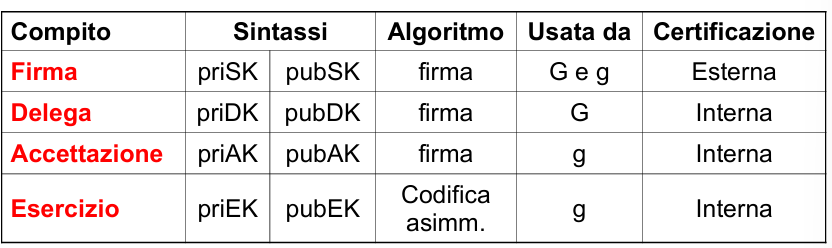
\includegraphics[width=0.7\linewidth]{Images/capitolo_4/chiavi_per_firma.png}
\end{figure}
Queste chiavi avranno una certificazione "interna" cioè sono \textbf{firmate tramite le chiavi di firma già certificate di G e g} di fatto, estendendo la PKI esistente. Queste saranno chiavi che avranno senso in funzione del fatto che sono certificate da delle chiavi già certificate.
Il protocollo si sviluppa dunque come segue:
\begin{align*}
    &1. G \to g: (G,g,\Omega,pubDK_G)_{Sign_{priSK_G}}\\
    &2. g \to G: (g,\Omega, pubAK_g,pubEK_g)_{Sign_{priSK_g}}\\
    &3. G \to g: (g,G,\Omega, pubDK_G,pubEK_g,pubAK_g)_{Sign_{priDK_G}}
\end{align*}
Analizziamo anche qui il protocollo passo passo:
\begin{enumerate}
    \item Al primo passaggio, G chiede a g se questo vuole ottenere la delega riguardo al compito $\Omega$ da parte di G. Questo primo messaggio è firmato con la chiave privata di firma di G.
    \item Dopodiché g invia a G la conferma di accettazione della delega mostrando la chiave pubblica di accettazione della delega e mostrando la chiave pubblica con la quale intende esercitare il diritto di delega. 
    \item G a questo punto conferma il tutto firmando la delega con la sua chiave privata di delega.
\end{enumerate}
Completato il protocollo, qualora g volesse esercitare il suo diritto di delega, dovrà fornire all'end-point il \textbf{token di delega} che non è altro che il messaggio 3 del protocollo, firmato con la chiave privata di accettazione di g:
\[\{(g,G,\Omega, pubDK_G,pubEK_g,pubAK_g)_{Sign_{priDK_G}}\}_{Sign_{priAK_g}}\]
L'end-point fungerà dunque da verificatore passivo, dovrà solo verificare che le firme nel token corrispondano alle chiavi scambiate.
Verifichiamo la possibilità di ottenere dei vantaggi da parte di uno o dell'altro:
\begin{itemize}
    \item Se G volesse ottenere un vantaggio su g, potrebbe terminare la sessione prima del messaggio 3. Tuttavia, non avrebbe modo di dimostrare che g abbia mai esercitato la delega poiché, per farlo, ha la necessità del token di delega che può generare solo g tramite le chiave privata di accettazione.
    \item Se g volesse ottenere un vantaggio potrebbe pensare di non andare avanti con il messaggio due, tuttavia anche in questo caso non ne otterrebbe nulla poiché non potrebbe esercitare la delega.
\end{itemize}
\subsubsection{Risoluzione delle controversie}
Vediamo cosa accade in caso di controversie:
\begin{itemize}
    \item Supponiamo G voglia negare di aver delegato g su $\Omega$. In tal caso g deve solamente mostrare il token di delega che, in quanto firmato con la chiave privata di delega di G, è effettivamente valida.
    \item Se g nega di aver accettato da G la responsabilità su $\Omega$, allora a G basta esibire il messaggio 2. Questo, per quanto possa sembrare un vantaggio, non lo è in realtà nel caso in cui manchi una prova che g abbia esercitato $\Omega$.
    \item Se g nega di aver esercitato $\Omega$ per conto di G, allora G insieme all'end-point mostra il messaggio 2 e il token di delega richiesto dall'end-point.
\end{itemize}
\subsection{Semplificazione del Protocollo}
Dal punto di vista della funzionalità, il protocollo in realtà funziona benissimo anche con le sole due chiavi di G e g. Questo perché potremmo scrivere il protocollo come segue:
\begin{align*}
    &1. G \to g: \text{Sign}_{priSK_G}(G, g, \Omega)\\
    &2. g \to G: \text{Sign}_{priSK_g}(g, \Omega)\\
    &3. G \to g: \text{Sign}_{priSK_G}(G, g, \Omega, Ev\_msg2)
\end{align*}
Infatti con il primo messaggio G chiede a g se vuole la delega, con il secondo g "accetta" la delega mentre con il terzo G dice che da quel momento la delega è attiva. Infatti, verrà prodotto il token che viene presentato all'end-point come segue:
\[\{Sign_{priSK_G}(msg3)\}_{priSK_g}\]

L'uso di chiavi dedicate ($DK$, $AK$, $EK$) serve a soddisfare principi di sicurezza che vanno oltre il semplice non-ripudio:
\begin{itemize}
    \item \textbf{Separazione dei Privilegi (Key Separation)}: Usare la chiave primaria ($SK$) per ogni singola operazione è rischioso. Se la chiave usata per firmare i token di delega venisse compromessa, in un sistema a chiavi separate avresti compromesso solo la capacità di delegare ($DK$). Nella versione semplificata, avresti compromesso l'intera identità digitale dell'utente ($SK$).
    \item \textbf{Limitazione del Rischio (Proxy Keys)}: Spesso il Grantee ($g$) deve usare la delega su macchine meno sicure o tramite software automatizzati. Usando una Execution Key ($EK_g$) creata ad hoc, $g$ non deve mai "caricare" la sua chiave primaria (molto preziosa) sul server che esegue il compito $\Omega$.
    \item \textbf{Prova di Intento Specifico}: Usando una Acceptance Key ($AK_g$), il Grantee genera una prova che non è solo una firma generica, ma un atto crittografico che significa esclusivamente "Accetto questa specifica delega". Questo previene attacchi di tipo Cross-Protocol Replay, dove una firma fatta per uno scopo viene riutilizzata per un altro.
    \item \textbf{Revocabilità Granulare}: È molto più facile revocare una singola chiave di delega ($DK_G$) o di esecuzione ($EK_g$) senza dover revocare il certificato principale dell'utente, cosa che richiederebbe la pubblicazione in una CRL (Certificate Revocation List) e avrebbe un impatto enorme.
\end{itemize}
